\documentclass{article}
\setlength{\oddsidemargin}{0.25 in}
\setlength{\evensidemargin}{-0.25 in}
\setlength{\topmargin}{-0.6 in}
\setlength{\textwidth}{6.5 in}
\setlength{\textheight}{8.5 in}
\setlength{\headsep}{0.75 in}
\setlength{\parindent}{0 in}
\setlength{\parskip}{0.1 in}

% ===== PACKAGES =====
\usepackage{amsmath,amssymb}
\usepackage{color}
\usepackage{subfigure}
\usepackage{mdframed}
\usepackage{changepage}
\newmdenv[
  topline=false,
  bottomline=false,
  skipabove=\topsep,
  skipbelow=\topsep
]{siderules}
\renewcommand{\abstractname}{}

% ===== VARIABLES =====
\def \R{\mathbb{R}}
\def \Pr{\mathbb{P}}
\def \D{{\rm D}}
\def \N{{\rm N}}
\def \xx{{\boldsymbol{\rm x}}}
\def \y{{\rm y}}




% ===== HEADER BOX =====
\newcommand{\lecture}[2]{
\pagestyle{myheadings}
\thispagestyle{plain}
\newpage
\noindent
\begin{center}
\rule{\textwidth}{1.6pt}\vspace*{-\baselineskip}\vspace*{2pt} % Thick horizontal line
\rule{\textwidth}{0.4pt}\\[1\baselineskip] % Thin horizontal line
\vbox{\vspace{2mm}
\hbox to 6.28in { {\bf CS 760: Machine Learning} \hfill Spring 2024 }
\vspace{4mm}
\hbox to 6.28in { {\Large \hfill #1  \hfill} }
\vspace{4mm}
\hbox to 6.28in { {\scshape Authors:}  #2 \hfill }}
\vspace{-2mm}
\rule{\textwidth}{0.4pt}\vspace*{-\baselineskip}\vspace{3.2pt} % Thin horizontal line
\rule{\textwidth}{1.6pt}\\[\baselineskip] % Thick horizontal line
\end{center}
\vspace*{4mm}
}

% ===== Jed's Defined Stuff ======
\DeclareMathOperator*{\argmin}{arg\!\min}
\DeclareMathOperator*{\argmax}{arg\!\max}
\usepackage{siunitx}
\usepackage{enumitem} % used to make alphabetical lists instead of numbered ones
\usepackage{mathtools}
\usepackage{graphicx}
\usepackage{caption}
\usepackage{hyperref}


% =============== DOCUMENT ===============
\begin{document}
\lecture{Convolutional Neural Networks}{Jed Pulley \& Keshav Sharan Pachipala}

\begin{center}
{\Large {\sf \underline{\textbf{DO NOT POLLUTE!}} AVOID PRINTING, OR PRINT 2-SIDED MULTIPAGE.}}
\end{center}

% \begin{abstract}
% Write your abstract here
% \end{abstract}

\section{Introduction}
    In recent years, Convolutional Neural Networks (CNNs) have emerged as a cornerstone technology in the field of deep learning, particularly in the domain of computer vision. CNNs are adept at extracting intricate patterns and features from spatially structured data. Some fields that benefit from CNNs include:
        \begin{enumerate}
            \item Image Classification
            \item Object Detection
            \item Medical Image Analysis
        \end{enumerate}
    
    In this paper, we won't go into the exact specifics of what a convolution is since it's slightly different in the discrete and continuous cases, as well as slightly different in a CNN context, but if you're really curious about it, 3Blue1Brown has some excellent videos visually explaining the mathematical concepts behind a convolution in his videos linked below [1] and [2].

\section{Understanding the Architecture}
    \subsection{NNs vs CNNs}
        CNNs and Neural Networks are similar in many ways, but also have drastically different architectures. From a high level, the classic neural network is shown as an input layer of neurons, a hidden layer, and an output layer, shown below:
        \begin{center}
            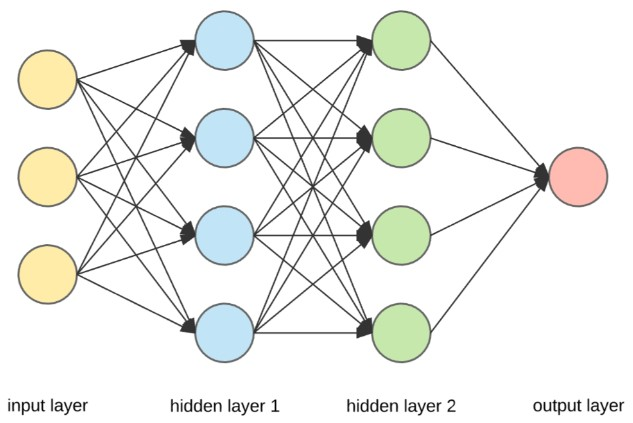
\includegraphics[scale=0.6]{images/NN.jpg}    
        \end{center}

        However, the architecture of a convolution neural network looks much different. There isn't one right way to structure it, but typically a CNN will have the input, a few convolution and pooling layers, a flattening step, and then finally a fully connected layer that leads to an output, as shown below:
        \begin{center}
            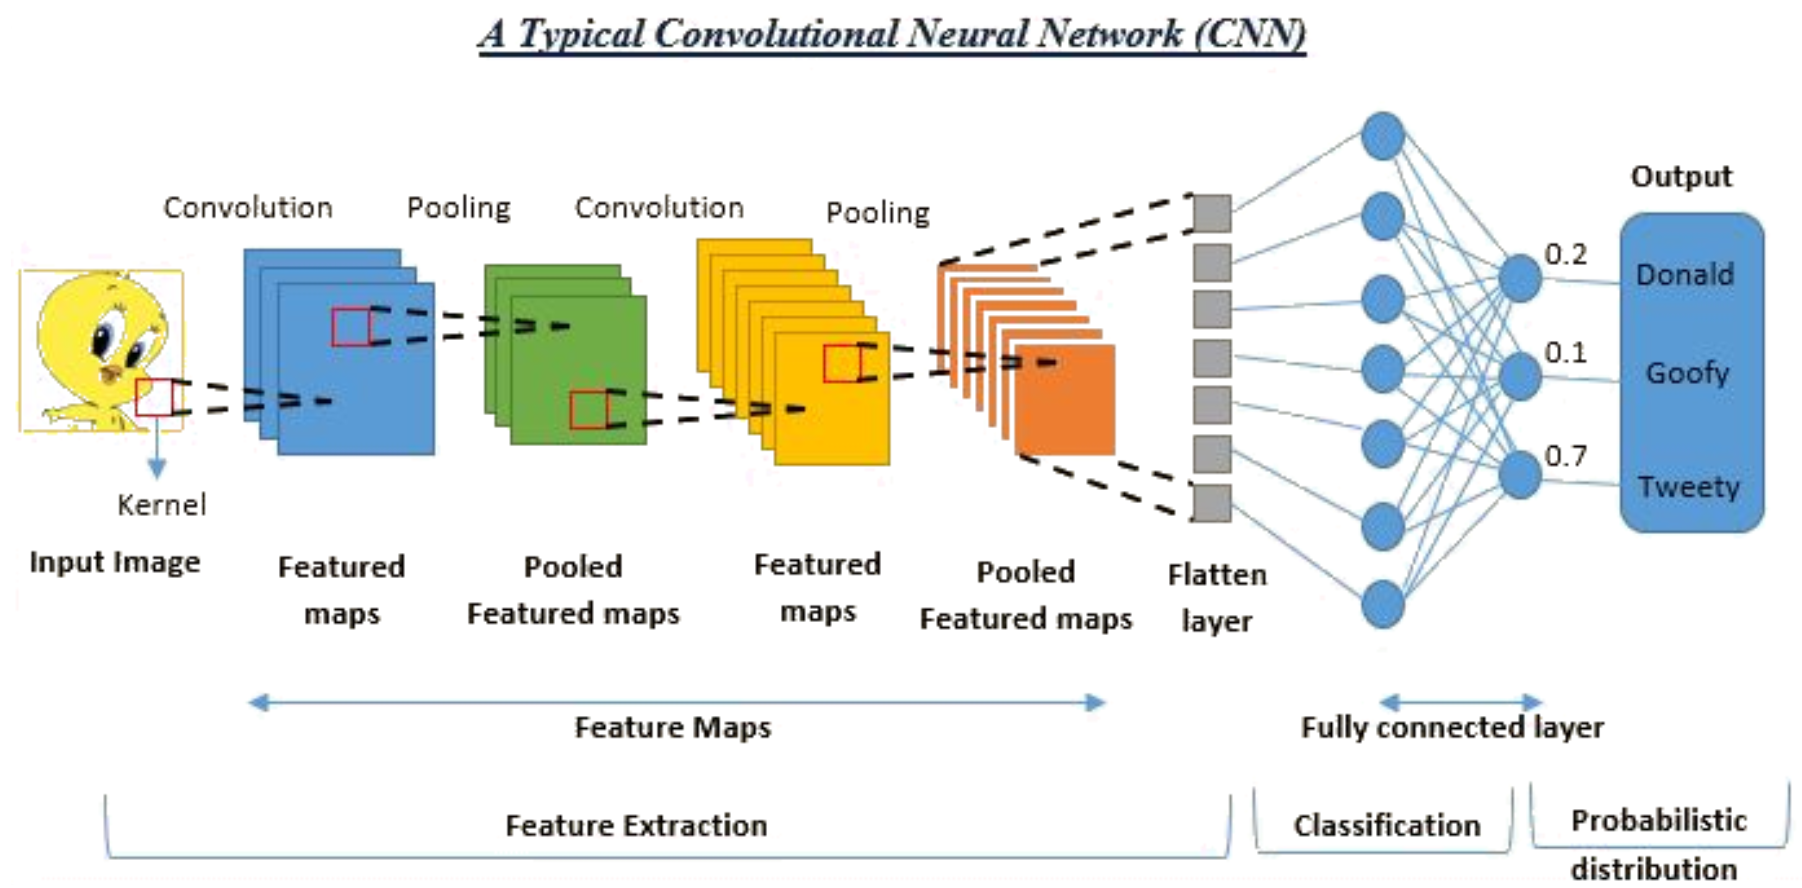
\includegraphics[scale=0.6]{images/CNN.jpg}
        \end{center}
        How you structure your CNN is an area of active research today. However, the above is a completely valid example.

    \subsection{Kernels}
        Fundamental to the idea of convolutions are kernels. In the 2D image processing case, a kernel often takes the form of a 3x3 grid of numbers that are "convolved" with the image. This convolution step means sliding the kernel across the image pixel by pixel, multiplying each element with it's overlapping counterpart, summing them up, and then dividing them by the kernel size (3x3 having a size of 9). The output is a single pixel in the output image/matrix. You scroll through the entire image performing the same operation until complete. Since the operative pixel is the center of the kernel, convolution runs into the issue of overlapping the image. So to avoid this, with a 3x3 kernel for example, a single pixel of padding is added to the image so that the kernel will fit in the first row/column.
        \begin{center}
            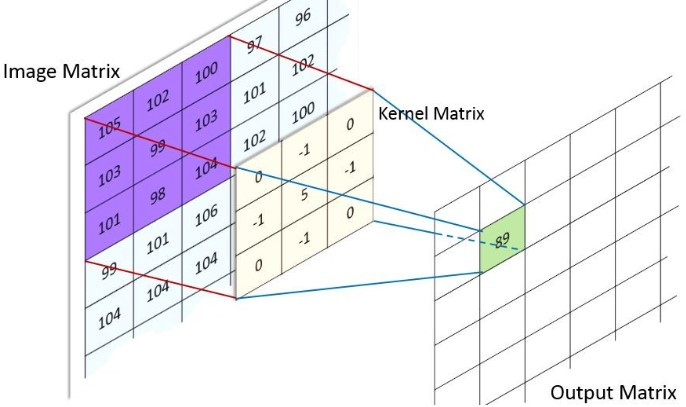
\includegraphics[scale=0.6]{images/kernel.jpg}
        \end{center}
    \subsection{Layers}
        \begin{enumerate}[label=(\alph*)]
            \item Convolution Layer
            The convolution layer is the most fundamental aspect of a CNN.
            \item Pooling Layer
            \item Flattening Layer
            \item Fully Connected Layer
            \item Output Layer                
        \end{enumerate}

    \subsection{Feature Hierarchy}
    
\section{Advanced CNN Architectures}
    \begin{enumerate}[label=(\alph*)]
        \item VGGNet
        \item ResNet
        \item Inception Network
    \end{enumerate}
    
\section{Future Directions and Trends}
    \begin{enumerate}[label=(\alph*)]
        \item TO-DO
        \item TO-DO
        \item TO-DO
    \end{enumerate}

\section{Resources}
    \textbf{[1]} 3Blue1Brown - But What is a Convolution? \\
    \url{https://www.youtube.com/watch?v=KuXjwB4LzSA&t=1s}
    
    \textbf{[2]} 3Blue1Brown - Convolutions | Why X+Y in probability is a beautiful mess \\
    \url{https://www.youtube.com/watch?v=IaSGqQa5O-M}
    
    \textbf{[3]} far1din - Convolutional Neural Networks from Scratch | In Depth \\
    \url{https://www.youtube.com/watch?v=jDe5BAsT2-Y}
    
    \textbf{[4]} Younesi, A., Ansari, M., Fazli, M. A., Ejlali, A., Shafique, M., \& Henkel, J. (2024). A Comprehensive Survey of Convolutions in Deep Learning: Applications, Challenges, and Future Trends. arXiv preprint arXiv:2402.15490 \\
    \url{https://arxiv.org/abs/2402.15490}


\end{document}